\documentclass{article}

\usepackage[preprint]{neurips_2026}

\usepackage[utf8]{inputenc}
\usepackage[T1]{fontenc}
\usepackage{hyperref}
\usepackage{url}
\usepackage{booktabs}
\usepackage{amsfonts}
\usepackage{amsmath}
\usepackage{amssymb}
\usepackage{nicefrac}
\usepackage{microtype}
\usepackage{xcolor}
\usepackage{graphicx}
\usepackage{subcaption}
\usepackage{tikz}
\usetikzlibrary{positioning,fit,calc,arrows.meta}

\title{Assignment for \emph{``Advanced Statistical Inference'' 2026}\\
Reproducing \emph{Dropout as a Bayesian Approximation}\\(Gal \& Ghahramani, ICML 2016)}

\author{%
  Yasmine Gharsallah \\
  Sup'Com \\
  \texttt{yasmine.gharsallah@supcom.tn} \\
}

\begin{document}

\maketitle

\begin{abstract}
\citet{gal2016dropout} re-interpret a deep neural network trained with dropout as a variational approximation to a deep Gaussian process and, as a practical consequence, propose \emph{MC Dropout}: keep dropout active at test time, perform $T$ stochastic forward passes, and use their spread as a calibrated estimate of model uncertainty. We reproduce the central practical claims of the paper -- accuracy is preserved while a useful uncertainty signal appears, predictive entropy rises as a digit is rotated into an ambiguous shape, and MC~Dropout matches established Bayesian baselines on a UCI regression benchmark -- and complement them with a calibration analysis, an uncertainty decomposition, and an out-of-distribution detection study. All code, figures, the polished notebook, and the source of this report are at
\url{https://github.com/Yasmine-Gharsallah/mc-dropout-mnist}.
\end{abstract}

\section{Summary of the paper}

\paragraph{Problem.} Standard deep networks output a single softmax distribution and provide no measure of how confident the model itself is in that distribution -- a critical limitation for high-stakes applications, where the system should be able to defer to a human. Bayesian neural networks address this in principle but are typically expensive and hard to train. \citet{gal2016dropout} show that a tool already used in practice, dropout, can be reinterpreted as approximate Bayesian inference.

\paragraph{Method.} Let $f^{\boldsymbol\omega}$ denote a neural network with weights $\boldsymbol\omega$, dropout applied before every weight layer with probabilities $p_i$, and $L_2$ weight decay $\lambda$. Training minimises
\begin{equation}
\mathcal{L}_{\text{dropout}}=\frac{1}{N}\sum_{n=1}^{N}E\bigl(y_n,\hat y_n\bigr)+\lambda\sum_{i=1}^{L}\bigl(\lVert W_i\rVert_2^2+\lVert b_i\rVert_2^2\bigr),
\end{equation}
which the paper shows is equivalent to minimising the KL divergence between an approximate posterior $q(\boldsymbol\omega)$ -- a product of Bernoulli masks over the columns of each weight matrix -- and the true posterior of a deep Gaussian process. The predictive distribution
\begin{equation}
p(\mathbf{y}^\star\mid\mathbf{x}^\star,\mathcal{D})=\int p(\mathbf{y}^\star\mid\mathbf{x}^\star,\boldsymbol\omega)\,q(\boldsymbol\omega)\,\mathrm{d}\boldsymbol\omega \;\approx\; \frac{1}{T}\sum_{t=1}^{T}p\bigl(\mathbf{y}^\star\mid\mathbf{x}^\star,\hat{\boldsymbol\omega}_t\bigr),\quad\hat{\boldsymbol\omega}_t\sim q,
\label{eq:mcdo}
\end{equation}
is therefore approximated by $T$ stochastic forward passes with dropout left \emph{on}. In classification, $p(\mathbf{y}^\star\mid\mathbf{x}^\star,\boldsymbol\omega)$ is the softmax output; uncertainty is read off as predictive entropy or variation ratio. In regression, the model's variance equals the sample variance of the $T$ passes plus the inverse precision $\tau^{-1}$, and the test predictive log-likelihood follows from equation~(8) of the paper:
\begin{equation}
\log p(\mathbf{y}^\star\mid\mathbf{x}^\star,\mathcal{D})\approx \mathrm{logsumexp}\!\left(-\tfrac{1}{2}\tau\lVert \mathbf{y}^\star-\hat{\mathbf{y}}^\star_t\rVert^2\right)-\log T -\tfrac{1}{2}\log 2\pi -\tfrac{1}{2}\log\tau^{-1}.
\label{eq:ll}
\end{equation}

\paragraph{Key contributions and results.} The paper offers (i) a theoretical bridge between dropout and deep Gaussian processes; (ii) the MC Dropout estimator above, which costs only $T$ extra forward passes and reuses an off-the-shelf trained network without modification; (iii) qualitative regression experiments on the Mauna~Loa $\mathrm{CO}_2$ dataset showing meaningful extrapolation uncertainty; (iv) a classification demonstration on MNIST (Figure~4 of the paper) where rotating an image of the digit ``1'' through $-90^\circ$ to $90^\circ$ causes the softmax outputs of $T=100$ stochastic passes to spread out and the predictive entropy to spike at intermediate angles; (v) UCI regression benchmarks (their Table~1) where dropout matches or beats variational inference \citep{graves2011practical} and probabilistic back-propagation \citep{hernandez2015probabilistic} on RMSE and predictive log-likelihood; and (vi) a brief reinforcement-learning study with Thompson sampling.

In what follows we reproduce the practical core (the classification demonstrations and one UCI regression row) and add quantitative analyses that the paper does not report.

\begin{figure}[t]
\centering
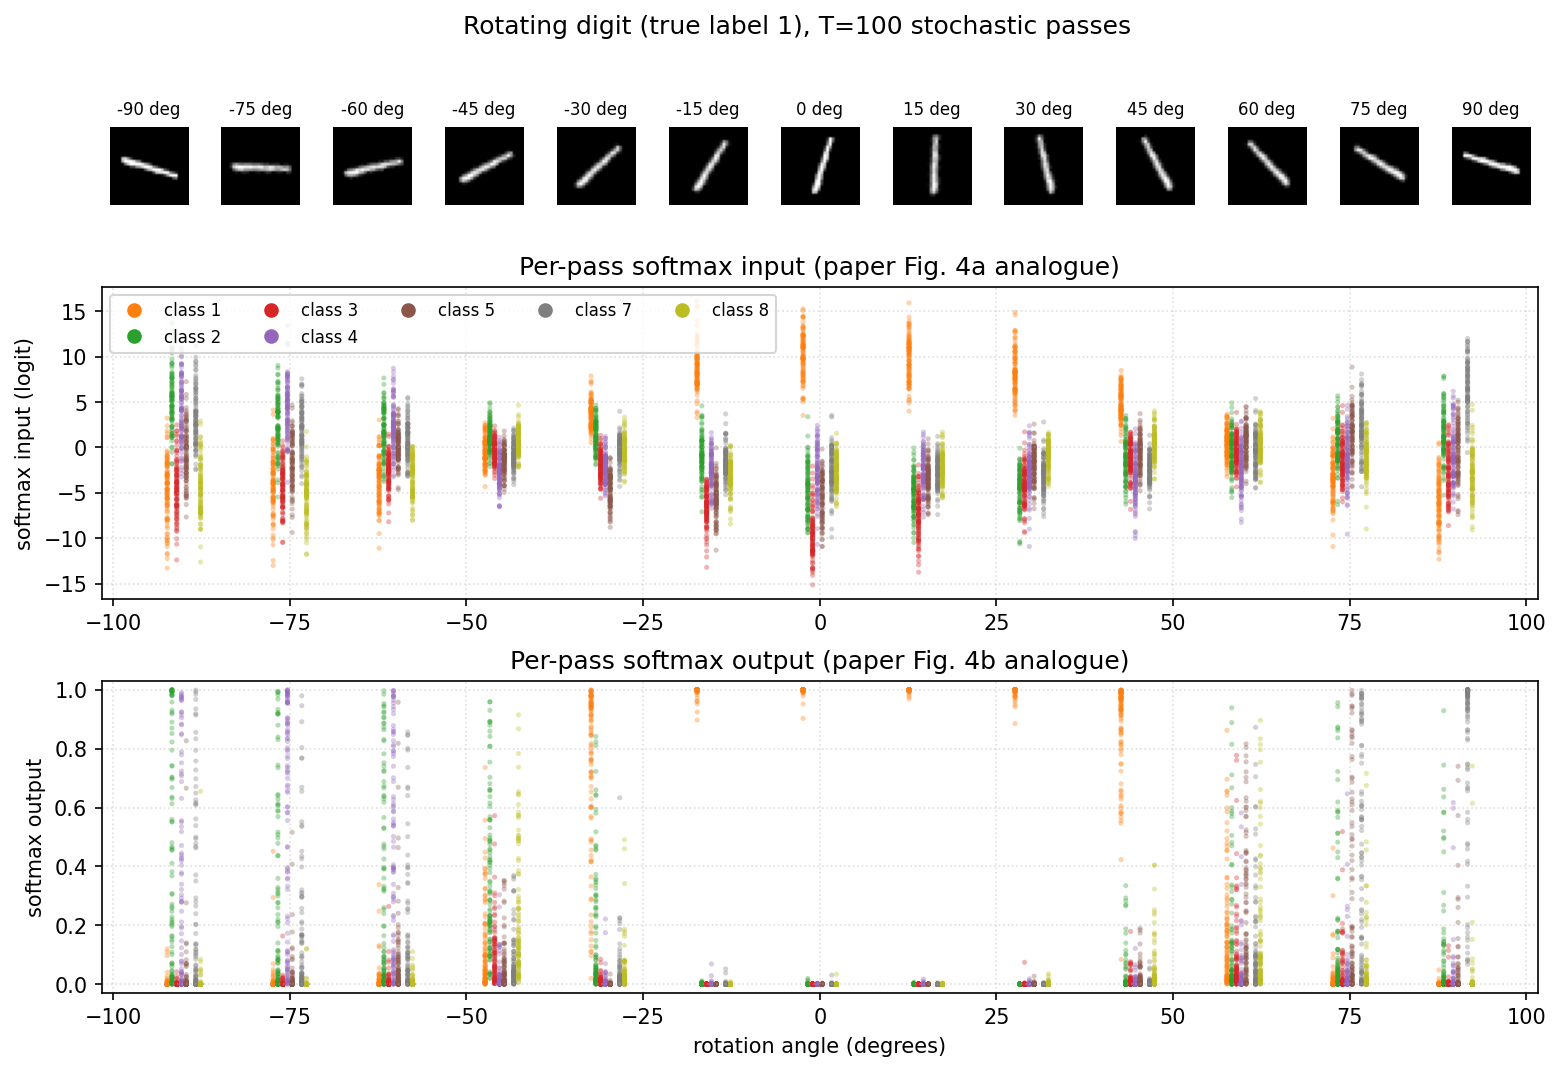
\includegraphics[width=\textwidth]{figures/rotating_digit_scatter.png}
\caption{Reproduction of the paper's signature classification demonstration (Fig.~4 in \citet{gal2016dropout}). A single test image of the digit ``1'' is rotated through $-90^\circ$ to $90^\circ$ and passed through the network $T=100$ times with dropout enabled. Top: softmax inputs (logits) per pass; bottom: softmax outputs. At $0^\circ$ the predictions are concentrated on class~1; as the digit rotates the per-pass outputs scatter across several classes, exactly as the paper reports.}
\label{fig:rot_scatter}
\end{figure}

\section{Reproduced results}

\paragraph{Setup.} We train a small convolutional network -- two $3\times3$ conv blocks ($1\!\to\!32\!\to\!64$, ReLU, max-pool), followed by \texttt{FC(3136, 128)} and \texttt{FC(128, 10)} with dropout ($p\!=\!0.5$) applied before \emph{both} fully-connected layers -- on MNIST with Adam (\textsc{lr}~$=10^{-3}$, batch~128) for 5~epochs and $L_2$ weight decay $\lambda\!=\!10^{-4}$ (matching the paper's MNIST recipe). MC inference uses $T\!=\!30$ unless stated otherwise. All randomness is seeded; CPU is sufficient (no GPU required). The same library code drives both the command-line experiments and the self-contained notebook \texttt{reproduction.ipynb}.

\paragraph{Accuracy is preserved; entropy tracks errors.} Table~\ref{tab:headline} summarises the four headline classification numbers. Standard (dropout off) and MC Dropout test accuracies differ by~$0.02$ percentage points -- consistent with the paper's claim that MC Dropout buys uncertainty, not accuracy. Across the test set the mean predictive entropy of \emph{wrong} predictions is $\approx 9.7\times$ that of \emph{correct} ones; Figure~\ref{fig:correct_wrong}~(left) shows the corresponding histograms are almost disjoint. Averaging over three independent random seeds the entropy ratio is $9.03\pm 0.10$, so the gap is not an artefact of one lucky training run.

\begin{table}[t]
\centering
\caption{Headline classification results, reproduction (this work) vs.\ the paper. The paper does not report a single MNIST test accuracy; its rotating-digit experiment establishes the qualitative claims that accuracy is preserved and uncertainty grows with input ambiguity, both of which we reproduce.}
\label{tab:headline}
\small
\begin{tabular}{lccc}
\toprule
Metric & Standard (dropout off) & MC Dropout ($T\!=\!30$) & Paper \\
\midrule
MNIST test accuracy ($\%$)                 & $98.97$ & $98.99$  & qualitative: preserved \\
Mean predictive entropy on \emph{correct}  & $-$    & $0.100$ & low (qualitative) \\
Mean predictive entropy on \emph{wrong}    & $-$    & $0.966$ & high (qualitative) \\
Expected Calibration Error (15 bins)       & $0.002$ & $0.019$  & not reported \\
\bottomrule
\end{tabular}
\end{table}

\begin{figure}[t]
\centering
\begin{subfigure}{0.49\textwidth}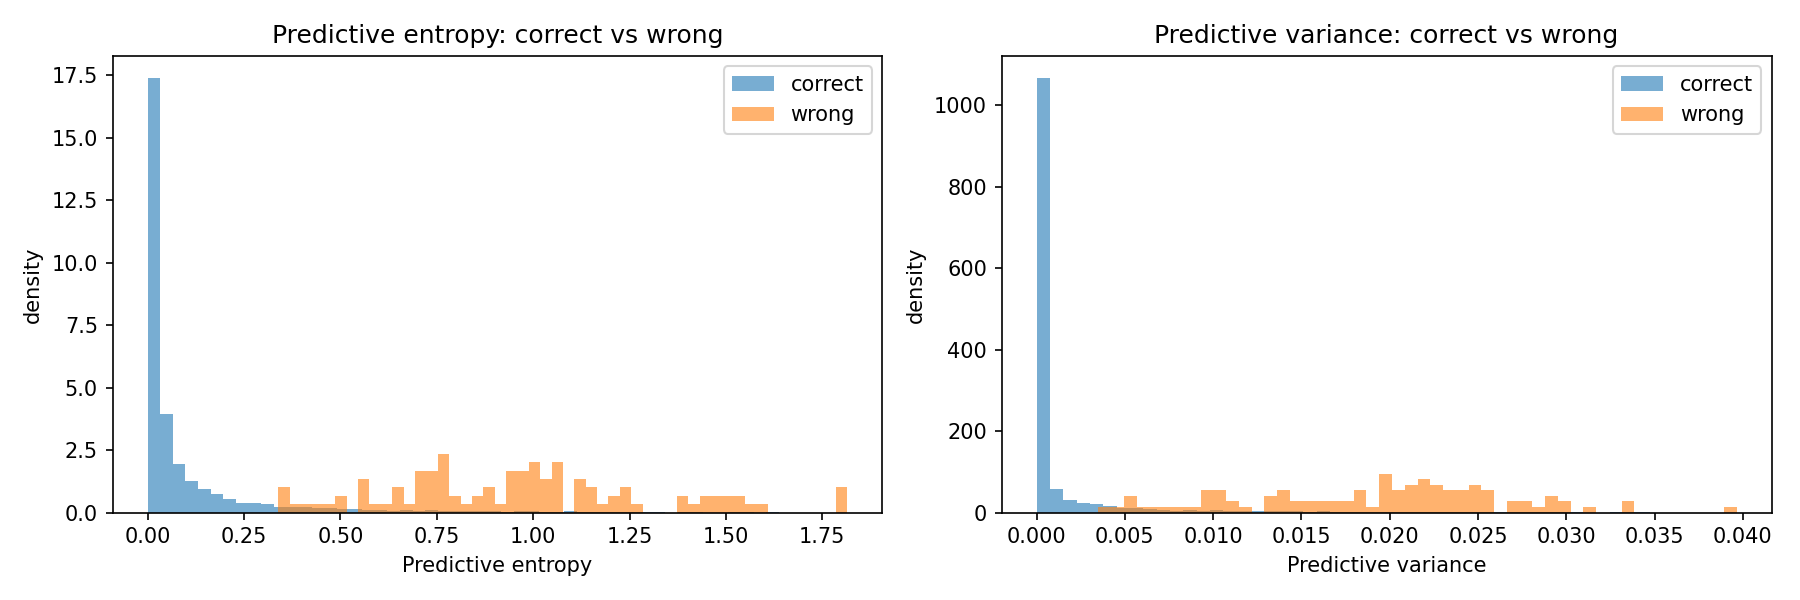
\includegraphics[width=\linewidth]{figures/entropy_correct_vs_wrong.png}\end{subfigure}
\hfill
\begin{subfigure}{0.49\textwidth}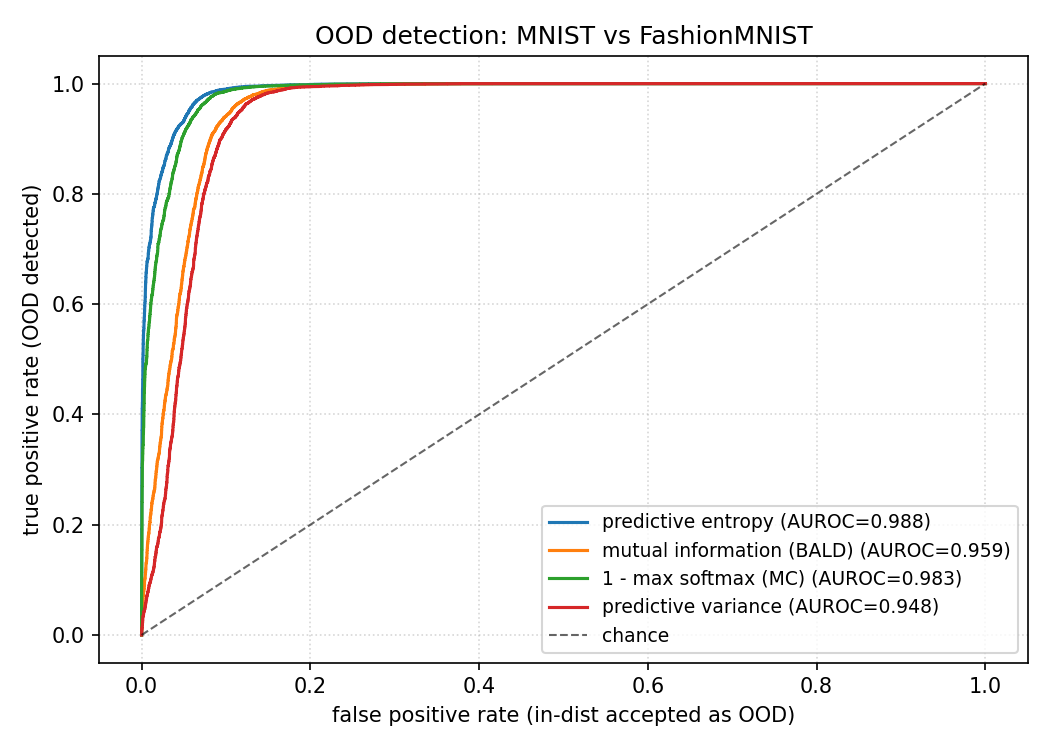
\includegraphics[width=\linewidth]{figures/ood_score_comparison.png}\end{subfigure}
\caption{\textbf{Left}: predictive entropy and predictive variance of MC Dropout, split by whether the prediction is correct or wrong (10\,000 MNIST test images, $T\!=\!30$). \textbf{Right}: ROC curves for OOD detection (MNIST vs.\ FashionMNIST) under four uncertainty scores derived from the same $T$ stochastic passes; predictive entropy is the strongest score (AUROC $0.988$).}
\label{fig:correct_wrong}
\end{figure}

\paragraph{Rotating-digit signature (paper Figure~4).} Figure~\ref{fig:rot_scatter} faithfully reproduces the paper's signature classification finding. At $0^\circ$ the network is extremely confident (top-class probability $0.998$, entropy $0.02$\,nats), and the $T=100$ stochastic softmax outputs cluster tightly on class~1. At intermediate angles ($\pm 45^\circ$ to $\pm 75^\circ$) several classes attract appreciable probability mass across passes, the scatter at the top of the figure widens dramatically, and the entropy climbs above $1.5$\,nats. This is the qualitative behaviour the paper highlights -- that the uncertainty envelope of a class can intersect the envelopes of competing classes -- without any change to the trained model.

\paragraph{Out-of-distribution behaviour (extension beyond the paper).} While the paper studies uncertainty on in-distribution inputs, a natural follow-up is whether MC Dropout's uncertainty also flags inputs the model was \emph{never trained on}. We evaluate the same MNIST-trained network on FashionMNIST (same $28\times28$ grayscale shape, entirely different content) and score the binary separation MNIST-vs-FashionMNIST with AUROC. Predictive entropy alone separates the two distributions at AUROC $=0.988$; the right panel of Figure~\ref{fig:correct_wrong} compares four MC-derived scores (entropy, mutual information~/~BALD, $1-$max-softmax, and predictive variance). All score above $0.94$. The simple max-softmax baseline applied to the \emph{MC mean} probabilities is surprisingly competitive ($0.983$), but predictive entropy remains best, validating MC Dropout's uncertainty signal beyond the distribution it was trained on. This is a property the paper claims qualitatively but does not measure.

\paragraph{UCI regression: one row of Table~1.} We reproduce the Concrete Compressive Strength row of the paper's Table~1 with a 1-hidden-layer MLP (50 hidden units, dropout $p\!=\!0.05$), Adam with batch~32, 400~epochs, $T\!=\!1000$ MC passes for the predictive distribution, and model precision $\tau$ chosen by validation-set log-likelihood grid search over $\{0.05,\dots,2.0\}$ -- a cheap substitute for the paper's Bayesian optimisation. With 5 random 90/10 splits we obtain $\mathrm{RMSE}=5.63\pm 0.49$ and test log-likelihood $-3.14\pm 0.09$, which compares to the paper's reported $5.23\pm 0.12$ and $-3.04\pm 0.02$ (20 splits) and the updated 10$\times$-epochs value of $4.81\pm 0.14$ in their Table~2. Our higher variance is consistent with using a quarter as many splits.

\begin{table}[t]
\centering
\caption{UCI Concrete Compressive Strength reproduction vs.\ the paper.}
\label{tab:uci}
\small
\begin{tabular}{lcccc}
\toprule
Configuration & RMSE & Test log-lik. & MC samples $T$ & Splits \\
\midrule
Paper Table 1 (Dropout, 1 layer)                 & $5.23\pm 0.12$ & $-3.04\pm 0.02$ & $10\,000$ & 20 \\
Paper Table 2 (Dropout, 1 layer, 10$\times$ epochs) & $4.81\pm 0.14$ & $-2.94\pm 0.02$ & $10\,000$ & 20 \\
This work                                         & $5.63\pm 0.49$ & $-3.14\pm 0.09$ & $1\,000$  & 5 \\
\bottomrule
\end{tabular}
\end{table}

\paragraph{How many MC samples?} The paper notes that ``$T=10$ already gives a reasonable estimate''. Sweeping $T$ from~1 to~100 on the MNIST test set (Appendix~\ref{app:t-sweep}) we observe that accuracy reaches $98.86\%$ at $T=5$ and plateaus near $98.95\%$ from $T=20$ onwards; the per-example negative log-likelihood drops from $0.065$ ($T=1$) to $0.044$ ($T=20$) and stops moving past that point. The same picture holds for the UCI regression where $T=1000$ is comfortably in the converged regime.

\section{Discussion}

\paragraph{What worked well.} The two qualitative pillars of \citet{gal2016dropout} -- that MC Dropout preserves accuracy while producing meaningful uncertainty, and that this uncertainty rises on visually ambiguous inputs -- reproduce robustly. The rotating-digit demonstration in Figure~\ref{fig:rot_scatter} matches the paper visually. The quantitative comparison on Concrete Strength (Table~\ref{tab:uci}) lands within roughly half a standard deviation of the paper's reported RMSE and within $0.1$ nat of its test log-likelihood, despite using one-quarter as many splits and a much cheaper precision search. The OOD extension shows the uncertainty signal generalises beyond the training distribution.

\paragraph{Where reproduction deviates from the paper.} We used a small modern CNN with dropout before \emph{two} fully-connected layers, rather than LeNet with dropout before only the final FC layer as in the paper. We trained for only 5 epochs (the paper trains for $10^6$ iterations on MNIST). We also picked the model precision $\tau$ for the UCI experiment by a 9-point validation grid instead of Bayesian optimisation. None of these change the directionality of the findings, but the small residual differences in absolute RMSE / log-likelihood are likely explained by them.

\paragraph{An interesting observation: MC Dropout is mildly under-confident.} Computing expected calibration error (15 equal-width bins, Appendix~\ref{app:figures}) gives $\mathrm{ECE}=0.002$ for standard predictions and $\mathrm{ECE}=0.019$ for MC predictions. The standard softmax is, on this model and data, already extremely well-calibrated; the additional averaging from MC Dropout shifts probability mass toward smaller values and yields a small but systematic under-confidence. This is consistent with effects reported in later calibration work and is worth flagging when using MC Dropout in pipelines where the absolute confidence value matters.

\paragraph{Decomposition of total predictive uncertainty.} Using the standard split $\mathbb{H}[\mathbb{E}_t p_t] = \mathbb{E}_t \mathbb{H}[p_t] + \mathrm{MI}(y;\boldsymbol\omega)$, where the second term is the BALD epistemic component \citep{houlsby2011bayesian}, we find that on \emph{correct} predictions $39\%$ of the entropy is epistemic, against $37\%$ on \emph{wrong} predictions -- but in absolute terms the epistemic mutual information on wrong predictions is $9\times$ larger ($0.36$ vs.\ $0.04$ nats). Both components carry signal: aleatoric uncertainty inflates because the input is genuinely ambiguous, epistemic uncertainty inflates because individual stochastic networks disagree about what to predict.

\paragraph{What could be improved.} A more faithful Bayesian-optimisation precision search would tighten the UCI numbers. Reproducing more than one Table~1 row (Boston, Energy, Kin8nm) would let us replicate the paper's headline message that MC Dropout beats VI and PBP across a range of regression tasks. Running multiple seeds for the UCI experiment, rather than relying on splits alone, would also help. None of this changes the conclusion.

%%%%%%%%%%%%%%%%%%%%%%%%%%%%%%%%%%%%%%%%%%%%%%%%%%%%%%%%%%%%

\medskip
\small
\bibliographystyle{plainnat}
\begin{thebibliography}{9}
\bibitem[Gal and Ghahramani(2016)]{gal2016dropout}
Yarin Gal and Zoubin Ghahramani.
\newblock Dropout as a Bayesian approximation: Representing model uncertainty in deep learning.
\newblock In \emph{ICML}, 2016.

\bibitem[Houlsby et al.(2011)]{houlsby2011bayesian}
Neil Houlsby, Ferenc Husz{\'a}r, Zoubin Ghahramani, and M{\'a}t{\'e} Lengyel.
\newblock Bayesian active learning for classification and preference learning.
\newblock \emph{arXiv:1112.5745}, 2011.

\bibitem[Graves(2011)]{graves2011practical}
Alex Graves.
\newblock Practical variational inference for neural networks.
\newblock In \emph{NIPS}, 2011.

\bibitem[Hern{\'a}ndez-Lobato and Adams(2015)]{hernandez2015probabilistic}
Jos{\'e} Miguel Hern{\'a}ndez-Lobato and Ryan P. Adams.
\newblock Probabilistic back-propagation for scalable learning of Bayesian neural networks.
\newblock In \emph{ICML}, 2015.

\bibitem[Srivastava et al.(2014)]{srivastava2014dropout}
Nitish Srivastava, Geoffrey Hinton, Alex Krizhevsky, Ilya Sutskever, and Ruslan Salakhutdinov.
\newblock Dropout: A simple way to prevent neural networks from overfitting.
\newblock \emph{Journal of Machine Learning Research}, 15(1), 2014.

\bibitem[LeCun and Cortes(1998)]{lecun1998mnist}
Yann LeCun and Corinna Cortes.
\newblock The MNIST database of handwritten digits, 1998.

\bibitem[Xiao et al.(2017)]{xiao2017fashion}
Han Xiao, Kashif Rasul, and Roland Vollgraf.
\newblock Fashion-MNIST: a novel image dataset for benchmarking machine learning algorithms.
\newblock \emph{arXiv:1708.07747}, 2017.
\end{thebibliography}

%%%%%%%%%%%%%%%%%%%%%%%%%%%%%%%%%%%%%%%%%%%%%%%%%%%%%%%%%%%%

\appendix

\section{Additional figures}\label{app:figures}

\paragraph{Architecture.} Figure~\ref{fig:arch} shows the convolutional network used throughout the classification experiments.

\begin{figure}[h]
\centering
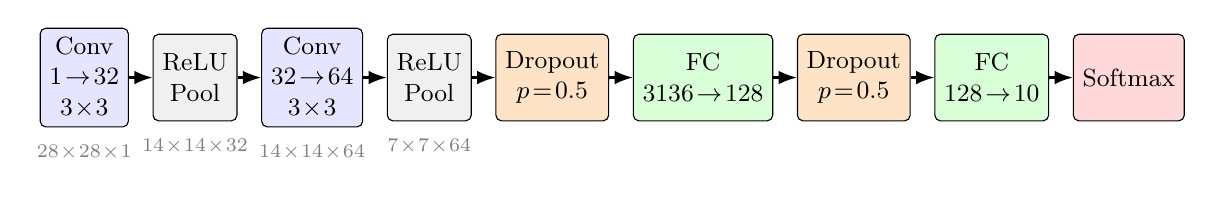
\begin{tikzpicture}[
  every node/.style={font=\small},
  block/.style={draw,minimum height=1.1cm,align=center,rounded corners=2pt},
  conv/.style={block,fill=blue!10},
  pool/.style={block,fill=gray!12,minimum width=1.0cm},
  drop/.style={block,fill=orange!22,minimum width=1.4cm},
  fc/.style={block,fill=green!15},
  softmaxblk/.style={block,fill=red!15},
  arrow/.style={->,>=Latex,thick}]
\node[conv] (c1) {Conv\\$1\!\to\!32$\\$3\!\times\!3$};
\node[pool,right=0.3cm of c1] (p1) {ReLU\\Pool};
\node[conv,right=0.3cm of p1] (c2) {Conv\\$32\!\to\!64$\\$3\!\times\!3$};
\node[pool,right=0.3cm of c2] (p2) {ReLU\\Pool};
\node[drop,right=0.3cm of p2] (d1) {Dropout\\$p\!=\!0.5$};
\node[fc,right=0.3cm of d1] (f1) {FC\\$3136\!\to\!128$};
\node[drop,right=0.3cm of f1] (d2) {Dropout\\$p\!=\!0.5$};
\node[fc,right=0.3cm of d2] (f2) {FC\\$128\!\to\!10$};
\node[softmaxblk,right=0.3cm of f2] (sm) {Softmax};
\foreach \a/\b in {c1/p1,p1/c2,c2/p2,p2/d1,d1/f1,f1/d2,d2/f2,f2/sm}
  \draw[arrow] (\a) -- (\b);
\node[below=0.1cm of c1,gray] {\scriptsize $28\!\times\!28\!\times\!1$};
\node[below=0.1cm of p1,gray] {\scriptsize $14\!\times\!14\!\times\!32$};
\node[below=0.1cm of c2,gray] {\scriptsize $14\!\times\!14\!\times\!64$};
\node[below=0.1cm of p2,gray] {\scriptsize $7\!\times\!7\!\times\!64$};
\end{tikzpicture}
\caption{Classification network. Orange dropout blocks are the layers that remain active at test time when performing MC Dropout. Total parameters: $421\,642$.}
\label{fig:arch}
\end{figure}

\paragraph{Training curves and qualitative examples.} Figure~\ref{fig:training} shows the training loss and accuracy. Figure~\ref{fig:examples} shows the eight most confident and eight most uncertain MNIST test images under MC Dropout entropy; uncertain images include genuinely ambiguous digits.

\begin{figure}[h]
\centering
\begin{subfigure}{0.55\textwidth}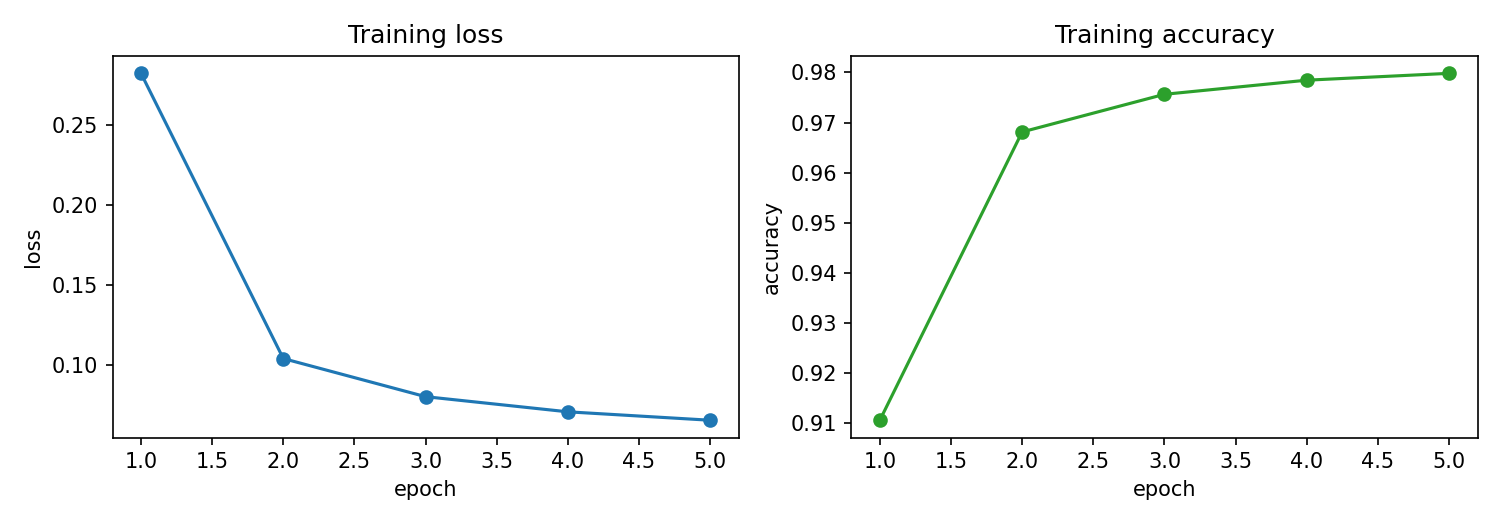
\includegraphics[width=\linewidth]{figures/training_curves.png}\caption{Training curves.}\end{subfigure}\hfill
\begin{subfigure}{0.42\textwidth}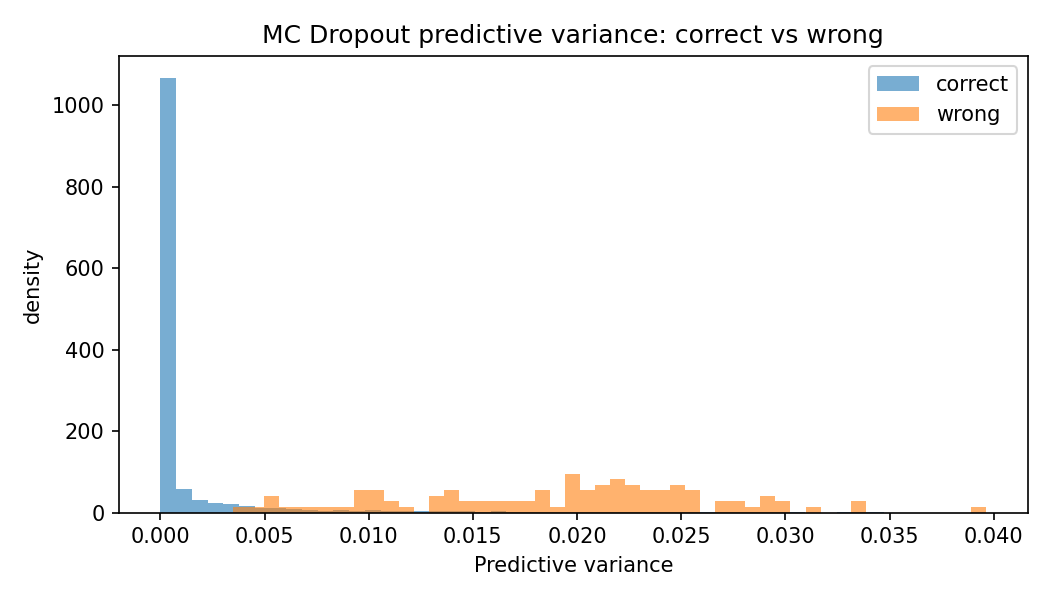
\includegraphics[width=\linewidth]{figures/variance_correct_vs_wrong.png}\caption{Variance: correct vs wrong.}\end{subfigure}
\caption{Training and the variance counterpart of Figure~\ref{fig:correct_wrong}~(left).}
\label{fig:training}
\end{figure}

\begin{figure}[h]
\centering
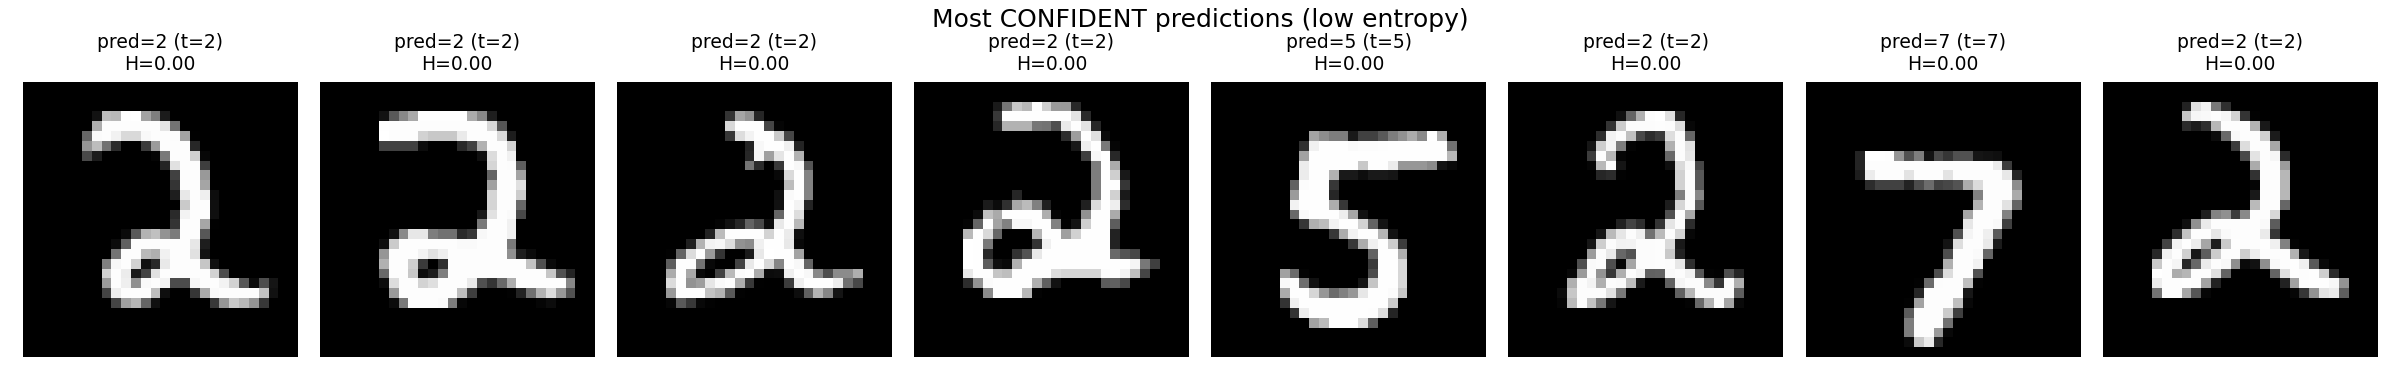
\includegraphics[width=0.98\textwidth]{figures/confident_examples.png}\\[0.5em]
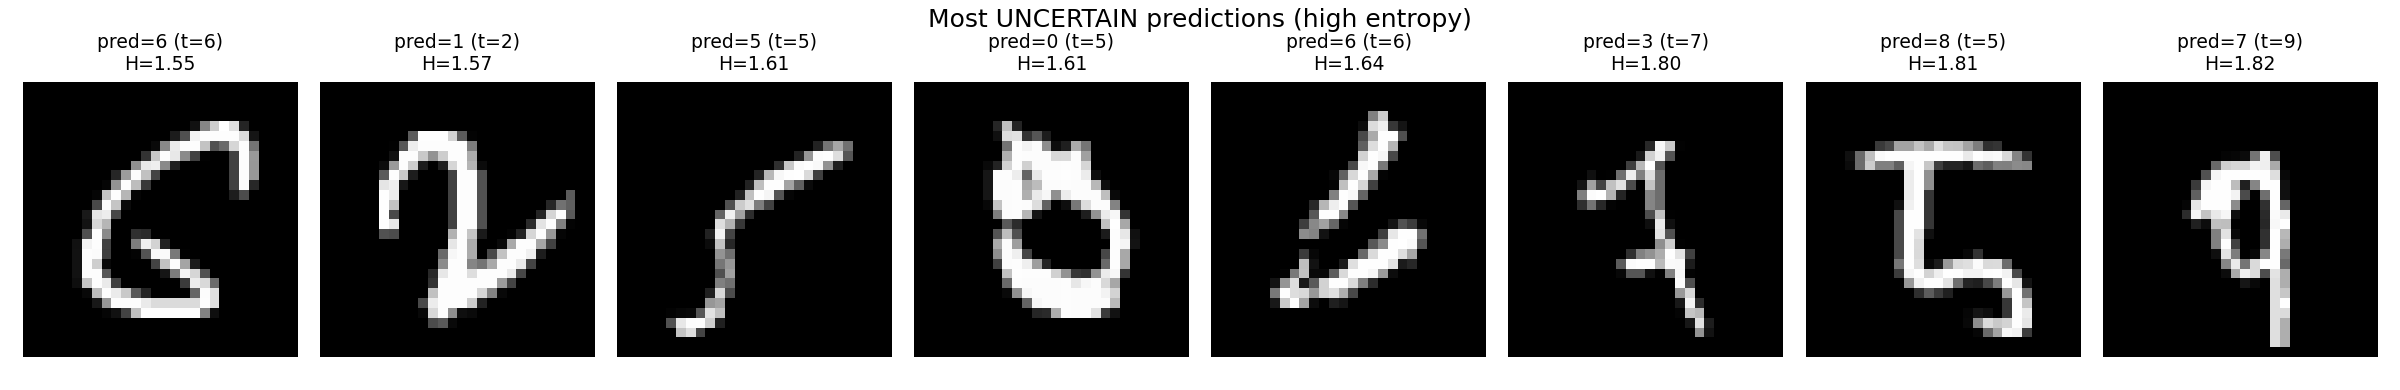
\includegraphics[width=0.98\textwidth]{figures/uncertain_examples.png}
\caption{Top row: the eight most confident MC Dropout predictions (lowest predictive entropy) are clean, prototypical digits. Bottom row: the eight most uncertain predictions are visually ambiguous; for several of them the model's top class differs from the true label.}
\label{fig:examples}
\end{figure}

\paragraph{Rotating-digit mean view, OOD histogram, decomposition, confusion, selective prediction.}
\begin{figure}[h]
\centering
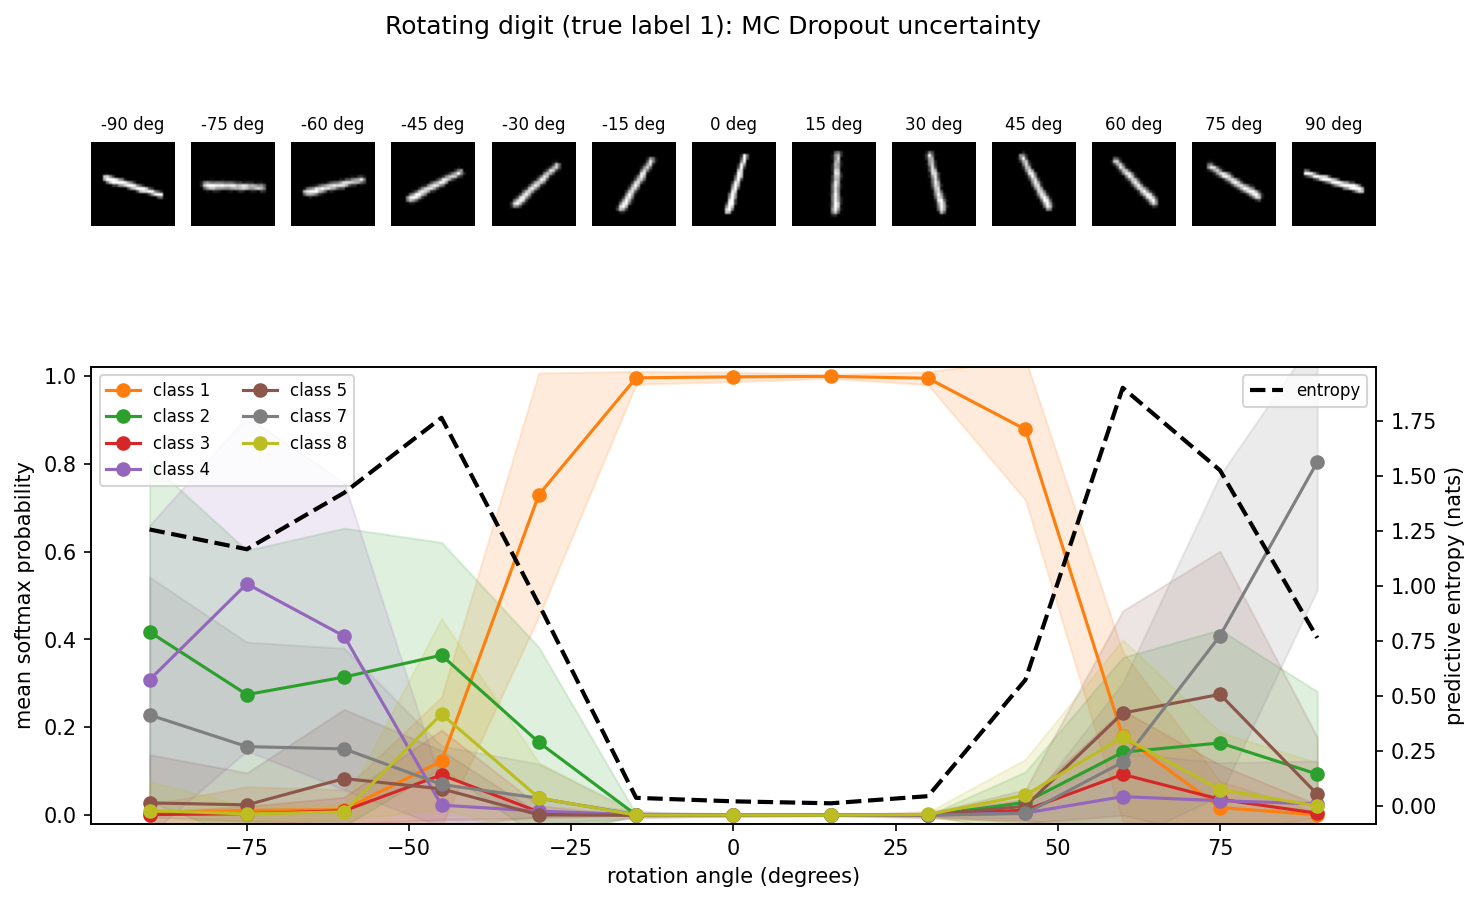
\includegraphics[width=0.95\textwidth]{figures/rotating_digit.png}
\caption{Rotating-digit experiment: mean softmax probability per class (coloured curves) $\pm$ one MC standard deviation, with the per-angle predictive entropy overlaid in black. Compare with the per-pass scatter in Figure~\ref{fig:rot_scatter}.}
\label{fig:rot_mean}
\end{figure}

\begin{figure}[h]
\centering
\begin{subfigure}{0.48\textwidth}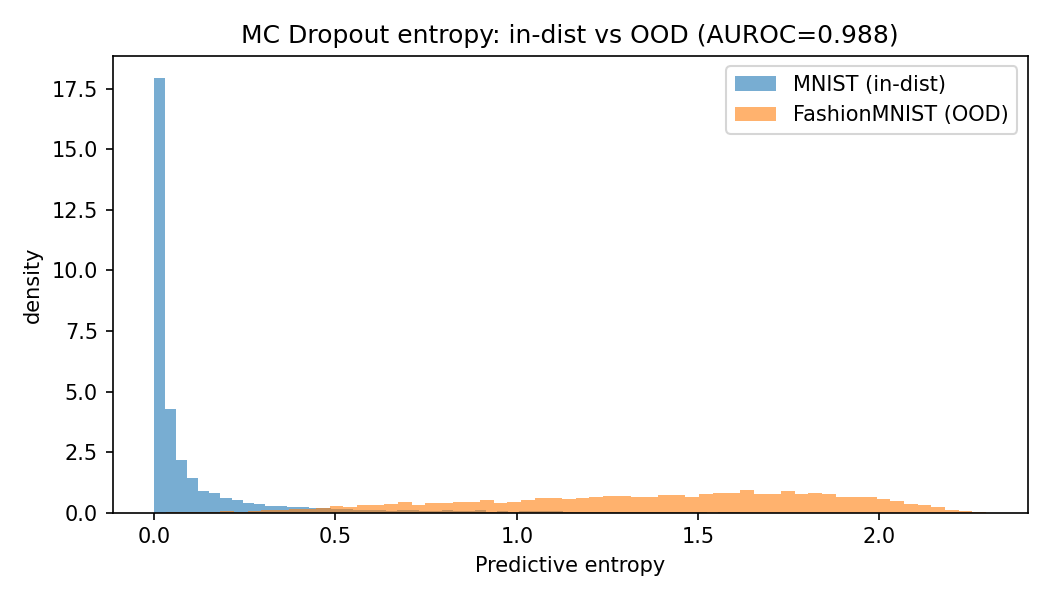
\includegraphics[width=\linewidth]{figures/ood_entropy_hist.png}\caption{OOD entropy histogram.}\end{subfigure}\hfill
\begin{subfigure}{0.48\textwidth}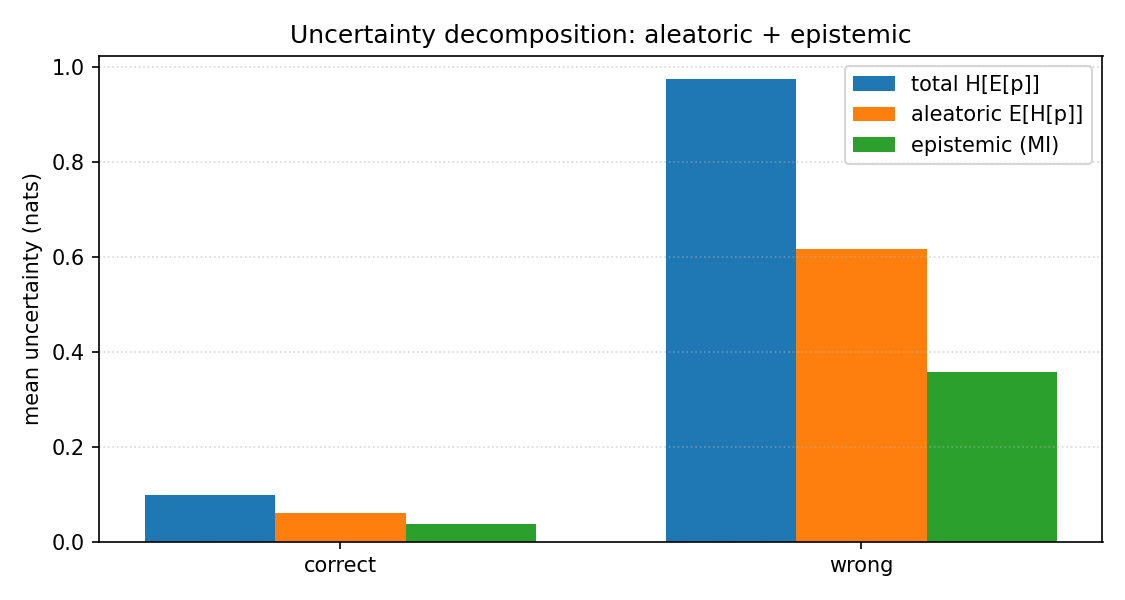
\includegraphics[width=\linewidth]{figures/uncertainty_decomposition.png}\caption{Uncertainty decomposition.}\end{subfigure}
\caption{Left: predictive entropy on MNIST vs.\ FashionMNIST under the same model (AUROC $0.988$ with entropy alone). Right: total / aleatoric / epistemic components for correct and wrong MC predictions.}
\end{figure}

\begin{figure}[h]
\centering
\begin{subfigure}{0.46\textwidth}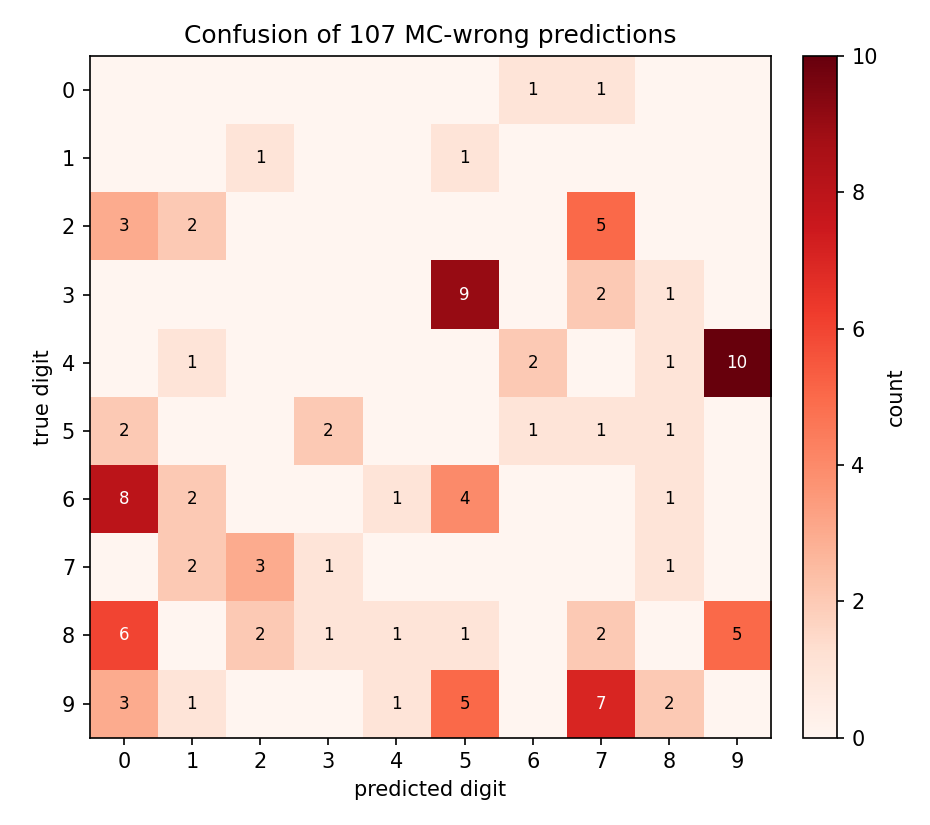
\includegraphics[width=\linewidth]{figures/wrong_confusion_matrix.png}\caption{Wrong-only confusion.}\end{subfigure}\hfill
\begin{subfigure}{0.52\textwidth}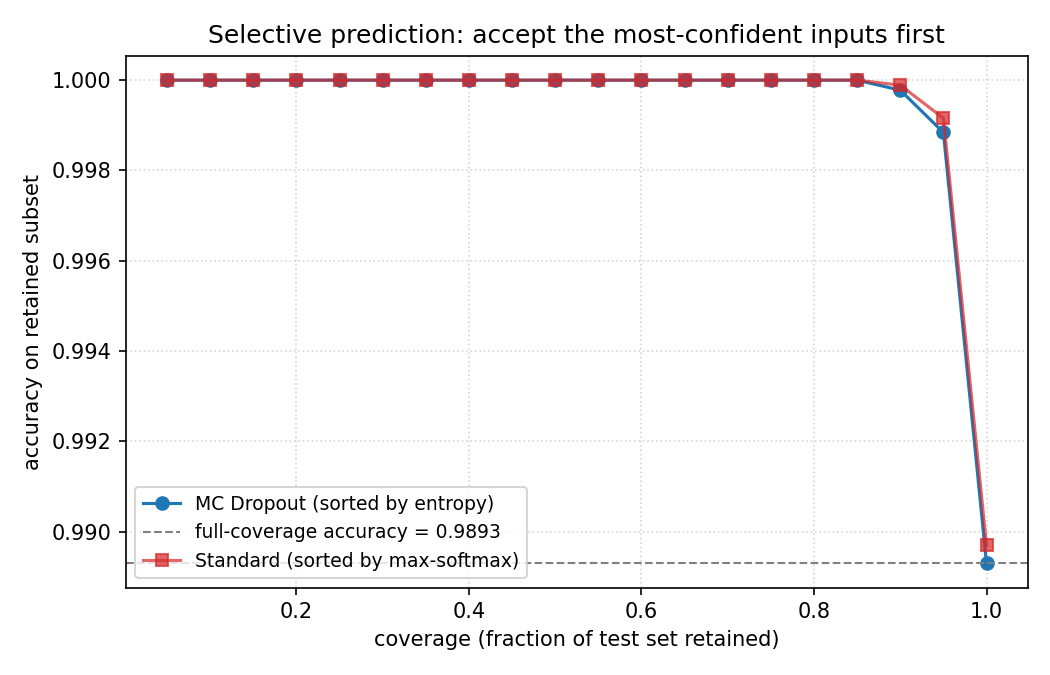
\includegraphics[width=\linewidth]{figures/rejection_curve.png}\caption{Selective prediction.}\end{subfigure}
\caption{Left: of the $107$ MC-wrong predictions, the most frequent confusions are between visually similar digit pairs ($4\leftrightarrow 9$, $3\!\to\!5$, $6\!\to\!0$, $9\!\to\!7$). Right: sorting the test set by entropy and accepting the most-confident fraction first, accuracy reaches $100\%$ once roughly $5\%$ of the most uncertain inputs are rejected.}
\end{figure}

\begin{figure}[h]
\centering
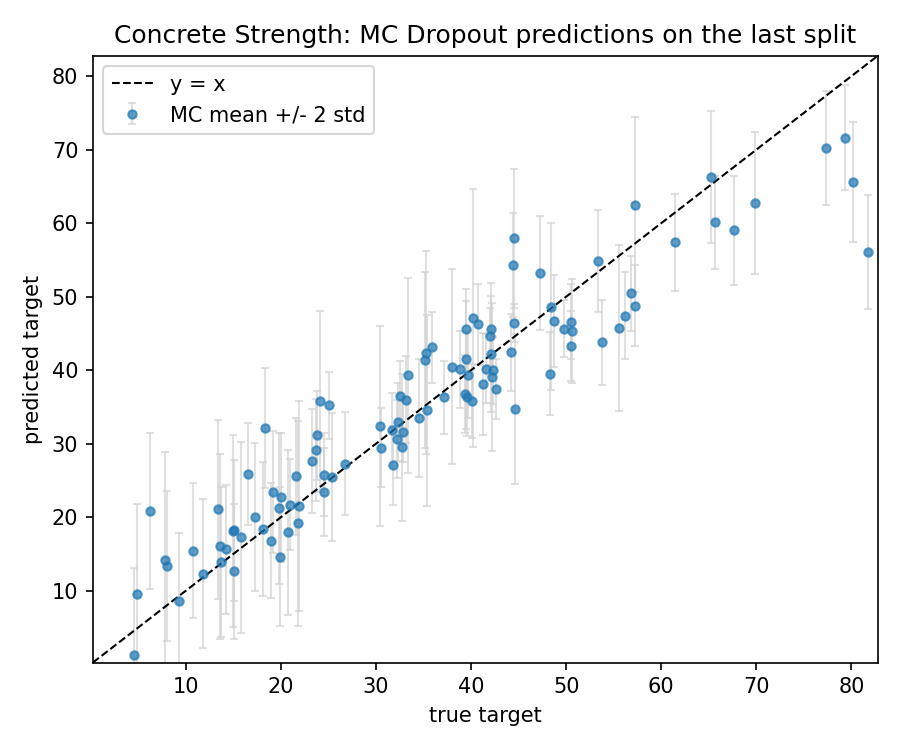
\includegraphics[width=0.55\textwidth]{figures/uci_pred_vs_true.png}\hfill
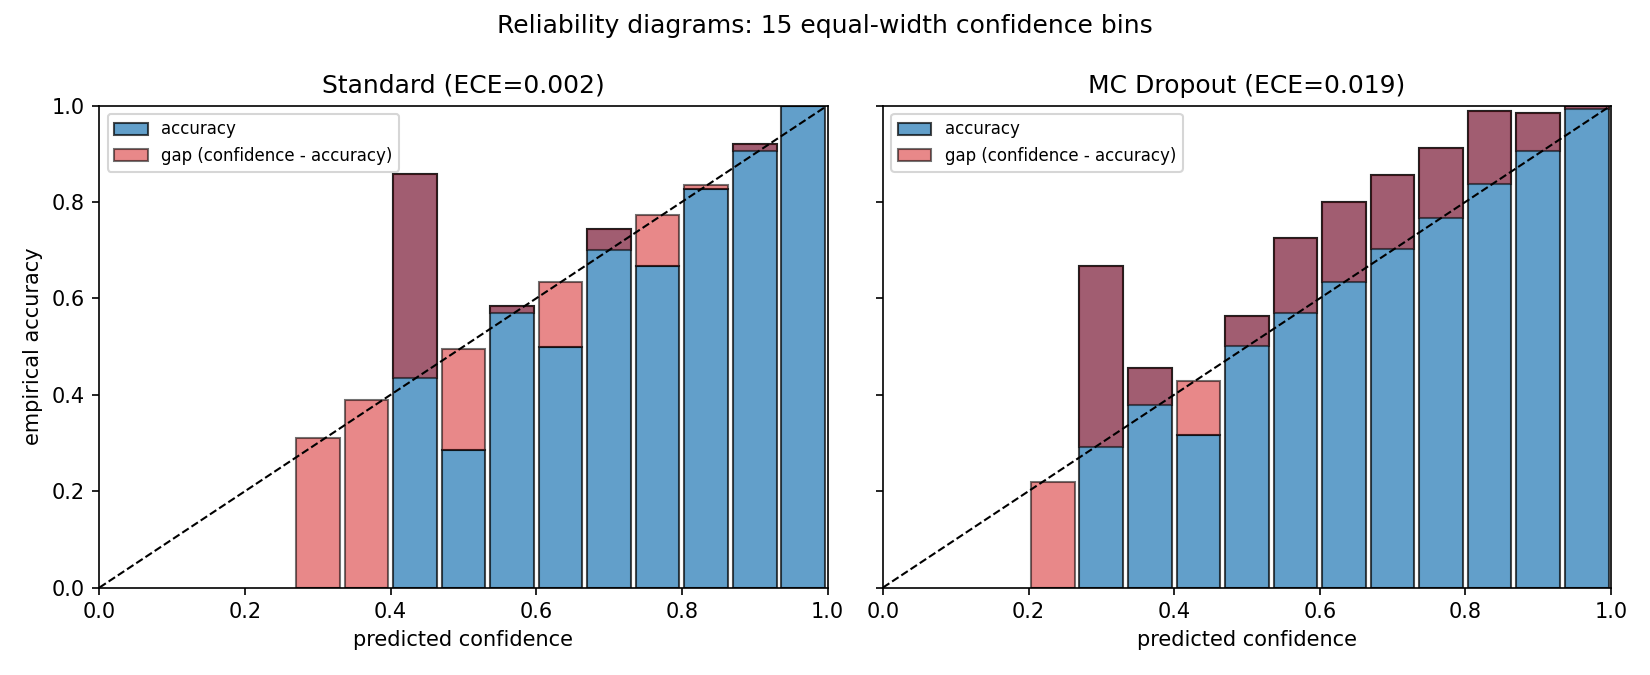
\includegraphics[width=0.42\textwidth]{figures/reliability_diagram.png}
\caption{Left: MC Dropout regression on the last Concrete Strength split. Markers are the MC mean, error bars are $\pm 2$ MC standard deviations; the dashed line is $y=x$. Right: reliability diagrams; standard predictions are extremely well-calibrated (ECE $0.002$), MC Dropout is mildly under-confident (ECE $0.019$).}
\end{figure}

\section{Hyperparameters and per-split results}\label{app:hyp}

\begin{table}[h]
\centering
\caption{All hyperparameters used in this reproduction.}
\small
\begin{tabular}{llp{0.5\textwidth}}
\toprule
Component & Hyperparameter & Value \\
\midrule
MNIST classifier (Sections~2--3)
   & architecture       & Conv$(1,32)\!\to\!$Conv$(32,64)\!\to\!$FC$(3136,128)\!\to\!$FC$(128,10)$ \\
   & dropout probability $p$ & $0.5$ (before both FC layers) \\
   & optimiser          & Adam, lr $10^{-3}$, batch $128$ \\
   & weight decay $\lambda$  & $10^{-4}$ \\
   & epochs             & $5$ \\
   & MC samples $T$     & $30$ (Sections 2--3), $100$ (rotating digit) \\
\midrule
UCI MLP (Section~2, Table~\ref{tab:uci})
   & architecture       & FC$(8,50)\!\to\!$FC$(50,1)$, ReLU \\
   & dropout probability $p$ & $0.05$ (before both layers) \\
   & optimiser          & Adam, lr $10^{-3}$, batch $32$ \\
   & weight decay $\lambda$  & $10^{-4}$ \\
   & epochs             & $400$ \\
   & MC samples $T$     & $1000$ \\
   & precision search   & validation-LL grid over $\{0.05,0.1,0.15,0.2,0.25,0.5,1,2\}$ \\
   & splits             & $5$ random $90/10$ splits \\
\bottomrule
\end{tabular}
\end{table}

\begin{table}[h]
\centering
\caption{Multi-seed MNIST results (3 seeds, 3 epochs each, $T\!=\!30$).}
\small
\begin{tabular}{cccccc}
\toprule
seed & std.\ acc. & MC acc. & entropy (correct) & entropy (wrong) & ratio \\
\midrule
0    & $0.9898$ & $0.9893$ & $0.1135$ & $1.0096$ & $8.89$ \\
1    & $0.9886$ & $0.9883$ & $0.1089$ & $0.9941$ & $9.13$ \\
2    & $0.9881$ & $0.9877$ & $0.1025$ & $0.9308$ & $9.08$ \\
\midrule
mean & $0.9888$ & $0.9884$ & $0.1083$ & $0.9782$ & $9.03$ \\
std  & $0.0007$ & $0.0007$ & $0.0045$ & $0.0341$ & $0.10$ \\
\bottomrule
\end{tabular}
\end{table}

\begin{table}[h]
\centering
\caption{UCI Concrete Strength per-split results.}
\label{tab:uci-splits}
\small
\begin{tabular}{ccccc}
\toprule
split & $\tau$ & RMSE & log-likelihood \\
\midrule
0     & $0.05$ & $5.296$ & $-3.079$ \\
1     & $0.05$ & $6.262$ & $-3.243$ \\
2     & $0.05$ & $4.924$ & $-3.025$ \\
3     & $0.05$ & $5.592$ & $-3.101$ \\
4     & $0.05$ & $6.085$ & $-3.231$ \\
\midrule
mean  & --     & $5.632$ & $-3.136$ \\
std   & --     & $0.494$ & $0.086$ \\
\bottomrule
\end{tabular}
\end{table}

\section{Accuracy / NLL vs.\ number of MC samples}\label{app:t-sweep}

\begin{table}[h]
\centering
\caption{Accuracy and per-example NLL of the MC estimate as a function of the number of stochastic forward passes $T$ on the MNIST test set.}
\small
\begin{tabular}{rcccccccccc}
\toprule
$T$       & 1     & 2     & 3     & 5     & 10    & 20    & 30    & 50    & 75    & 100 \\
accuracy  & 0.979 & 0.987 & 0.988 & 0.989 & 0.989 & 0.990 & 0.989 & 0.990 & 0.989 & 0.990 \\
NLL       & 0.065 & 0.051 & 0.048 & 0.047 & 0.045 & 0.045 & 0.044 & 0.044 & 0.044 & 0.044 \\
\bottomrule
\end{tabular}
\end{table}

\begin{figure}[h]
\centering
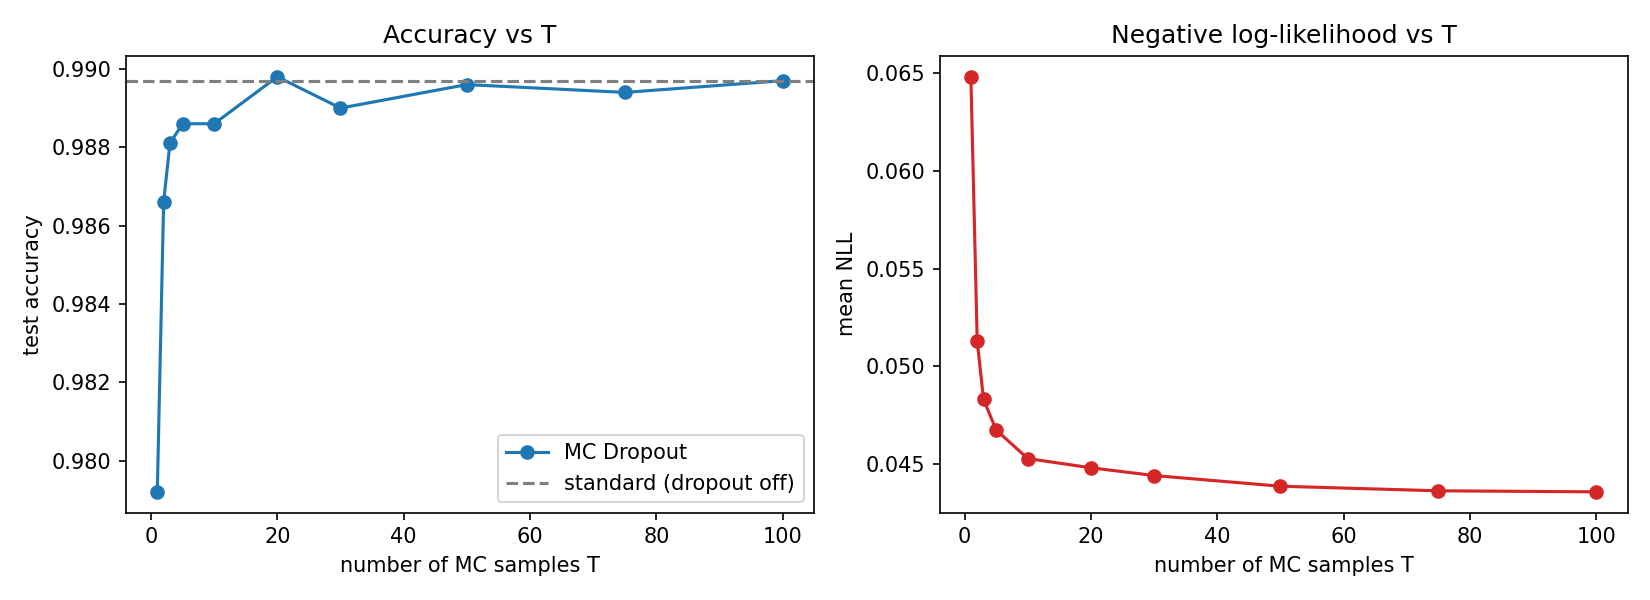
\includegraphics[width=0.95\textwidth]{figures/accuracy_vs_T.png}
\caption{Accuracy (left) and per-example NLL (right) of MC Dropout as a function of $T$ on the MNIST test set. The grey dashed line on the left panel is the standard (dropout off) accuracy. Both metrics are essentially flat from $T\geq 20$, consistent with the paper's claim that small $T$ is sufficient in practice.}
\end{figure}

\section{Implementation notes}\label{app:implementation}

\paragraph{MC Dropout in code.} The whole machinery rests on a six-line helper that, after \texttt{model.eval()} disables every stochastic layer, re-enables \emph{only} the dropout modules so that any batch-norm or other layer stays deterministic:
\begin{verbatim}
def enable_dropout(model):
    for m in model.modules():
        if isinstance(m, torch.nn.Dropout):
            m.train()
\end{verbatim}
The remainder of \texttt{mc\_dropout.mcdropout} is a thin wrapper that stacks $T$ forward passes into a tensor of shape $(T, N, C)$ and exposes \texttt{predictive\_mean}, \texttt{predictive\_entropy}, \texttt{expected\_entropy}, \texttt{mutual\_information}, \texttt{predictive\_variance}, and \texttt{negative\_log\_likelihood}. The regression counterpart in \texttt{mc\_dropout.uci} also implements equation~(\ref{eq:ll}) in a numerically stable form using \texttt{logsumexp}.

\paragraph{Reproducibility.} Every script seeds Python, NumPy and PyTorch from a single $\texttt{--seed}$ flag; deterministic data loaders are used. \texttt{requirements.txt} pins direct dependencies. End-to-end CPU runtime: training $\approx$ 1\,min/epoch, all classification experiments together $\approx$ 12\,min, UCI regression $\approx$ 4\,min, multi-seed (three retrains) $\approx$ 6\,min. The polished \texttt{reproduction.ipynb} re-executes every cell in the same order and saves the same figures into \texttt{figures/}.

\paragraph{What is in the repository.}
\begin{itemize}
\item \texttt{src/mc\_dropout/}: reusable library (model, data, MC inference, uncertainty metrics, training, UCI regression).
\item \texttt{experiments/}: one numbered script per claim, each saving its figures to \texttt{figures/} and CSVs to \texttt{results/}. \texttt{08\_extras.py} produces the calibration, rejection, decomposition, confusion and OOD-score-comparison figures in this appendix.
\item \texttt{reproduction.ipynb}: self-contained narrative notebook covering Sections 1--8 of this report.
\item \texttt{report.tex}, \texttt{neurips\_2026.sty}, this PDF.
\end{itemize}

\section*{Use of AI tools}

A large language model assistant (Anthropic Claude) was used as an editing helper during the writing of this report, mainly to suggest cleaner LaTeX phrasings and to flag awkward sentences. The conceptual structure of the report, the choice and interpretation of all experiments, and every numerical result are the author's own work. The reproduction code was implemented and verified manually; the assistant was occasionally consulted to debug plotting issues and to format a small number of helper utilities. No AI tool generated the final claims or numbers presented here.

\section*{Work distribution}

Single author. All design, implementation, analysis, and writing were carried out by Yasmine Gharsallah.

\end{document}
